\section{Análisis de sensibilidad  de una monocapa como biosensor}
\label{section:sensLambda}

En las secciones anteriores se estudió la respuesta EM de una monocapa desordenada de NPs esféricas e idénticas, soportada por un sustrato con índice de refracción $n_s=1.5$, simulando a un vidrio BK7, e inmersa en en agua (matriz con índice de refracción $n_m=1.33$). Cuando las NPs se iluminan en un configuración ATR, se observa un supuesto modo colectivo, el cual puede sintonizarse al seleccionar los siguientes parámetros: la fracción de cubierta $\Theta$ de la monocapa, el material de las NPs y el radio $a$ de éstas. En la Fig. \ref{fig:RT-AuAg} se muestran los resultados de la reflectancia de una monocapa de NPs de oro y una de NPs de plata, con los parámetros $a$ y $\Theta$ aptos para el biosensado. La elección de $a=30$ nm y $\Theta=0.125$ para las NPs de oro, y $a=40$ nm y $\Theta=0.1$ para las de plata, sintoniza al supuesto modo colectivo dentro del espectro visible y, al calcular al reflectancia a las longitudes de onda $\lambda^{exc}$ que excitan al supuesto modo colectivo, la reflectancia es mínima ($R\approx 0 $) para ángulos de incidencia menores a $80^\circ$ para polarización \emph{p} y \emph{s}.

Los biosensores plasmónicos miden cambios en el índice de refracción de la matriz y su rendimiento puede expresarse mediante la sensibilidad de bulto $S_B$ \cite{estevez2014trends,svedendahl2009refractometric}, que es la dependencia del corrimiento al rojo $\delta \lambda^{exc}$ de la excitación ante cambios en el índice de refracción de la matriz $\delta n_m$ medido en unidades de índice de refracción (Refractive Index Units, RIU),\index{Índice de refacción!Unidades de índice de refracción RIU} es decir
%
	\begin{equation}
	S_B = \frac{\delta \lambda^{exc}}{\delta n_m}.
	\label{eq:SBulk}
	\end{equation}
%
Otro parámetro que caracteriza el rendimiento del biosensor es la anchura a media altura (Full Width at Half Maximum, FWHM) $\Gamma$\index{Anchura a media altura (FWHM) ($\Gamma$)}. Para considerar tanto la sensibilidad de bulto como la FWHM en el rendimiento del biosensor, se define la \emph{figura de mérito} (Figure of Merit, FoM) de bulto  $\textit{FoM}_B$ dada por la expresión\index{Biosensor!Figura de Mérito (FoM)}\index{Biosensor!Figura de Mérito (FoM)!de bulto ($\textit{FoM}_B$)}
%
	\begin{equation}
	\textit{FoM}_B = \frac{S_B}{\Gamma}
			=\frac{1}{\Gamma}\frac{\delta \lambda^{exc}}{\delta n_m},
	\label{eq:FoM}
	\end{equation}
%
la cual se reporta evaluada en $n_m=1.33$. El empleo de la $\textit{FoM}_B$ permite tanto comparar  la sensibilidad como calificar la calidad de biosensores ópticos que emplean distintos tipos de resonancias \cite{svedendahl2009refractometric}, como puede ser la comparación entre sensores comerciales, basados en el plasmón polaritón de superficie (Surface Plasmon Polariton, SPP), el supuesto modo colectivo, predicho por del CSM, y los sensores basados en las resonancias de superfice localizadas (Localized Surface Plasmon Resonance, LSPRs), como las resonancias de una monocapa de nanodiscos desordenados \cite{svedendahl2009refractometric}, o las resonancias de red de plasmón de superficie (Plasmon Surface Lattice Resonances, PSLRs), estudiadas en \cite{kabashin2009plasmonic} y \cite{danilov2018ultra}.

\begin{figure}[b!]\centering
	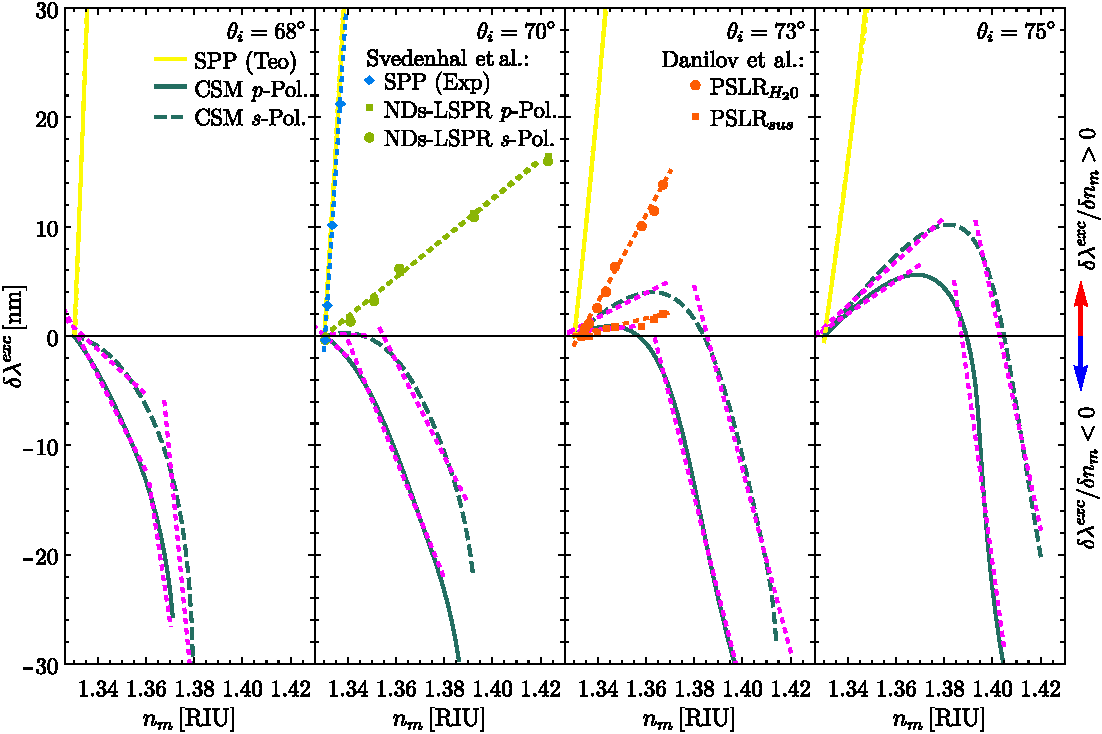
\includegraphics[width=\linewidth]{2-Resultados/figs/11-SPPCSM/1_comparacionAugtEye.pdf}\vspace*{-.7em}
	\caption{ Análisis de comportamiento del supuesto modo colectivo en una monocapa de NPs idénticas de oro ---radio $a=30$ nm y fracción de cubierta $\Theta=0.125$--- predicho por el CSM y  considerando $\theta_i=68^\circ,\, 70^\circ,\, 73^\circ$ y $75^\circ$. \textbf{a)} Corrimiento al rojo de la longitud de onda de excitación $\delta\lambda^{exc}$ como función del índice de la matriz $n_m$, para el supuesto modo colectivo para polarización  \emph{p} (CSM \textit{p}-Pol., líneas turquesas continuas) y \emph{s} (CSM \textit{s}-Pol., líneas turquesas discontinuas), para el SPP enn una película de oro de $50$ nm de grosor [SPP (Teo), líneas moradas; SPP (Exp), rombos azules], la NDs-LSPR  en una monocapa desordenada de NDs para polarización \emph{p} (ND \textit{p}-Pol., círculos verdes) y \emph{s} (ND \textit{s}-Pol., cuadrados verdes) y el SPLR medido cuan el haz de luz es refractado en la matriz (PSLR$_{H_{2}O}$, puntos naranjas) y en el sustrato (PSLR$_{sus}$, cuadrados naranjas). Los datos experimentales del SPP y de la NDs-LSPR corresponden a los resultados de Svedenhal et al. reportados en \cite{svedendahl2009refractometric} y los de las PSLR a los resultados de Danilov et al. reportados en \cite{danilov2018ultra}. Cuando $S_B=\delta\lambda^{exc}/\delta n_m>0$ el modo se corre hacia el rojo y cuando $S_B<0$, se corre al azul. Las líneas punteadas delgadas corresponden a aproximaciones lineas para determinar $S_B$ y sus valores es encuentran en la tabla  \ref{tab:SB}.}\label{fig:SensThetai}
	\end{figure}	

En la Fig. \ref{fig:SensThetai} se compara la sensibilidad del supuesto modo colectivo de una monocapa de NPs de oro ($a=30$ nm y $\Theta=0.125$) con la del SPP (para un película de oro de $50$ nm de grosor), así como con resultados experimentales de la sensibilidad del SPP ---reportada por  Svedenhal et al.\footnote{\label{fn:Motivacion}Ver capítulo \ref{chapter:Motivacion} para una descripción más detallada de sus resultados.} \cite{svedendahl2009refractometric} para una película de oro de $50$ nm de grosor a $\theta_i = 70^\circ$--- , con resultados experimentales de la sensibildad de un  arreglo bidimensional desordenado de nanodiscos (NDs)---reportado por Svedenhal et al.\textsuperscript{\ref{fn:Motivacion}}  \cite{svedendahl2009refractometric}, donde los NDs son nanocilindros de oro de $30$ nm de altura y $120$ nm de diámetro, para polarización \emph{p} y \emph{s} a $\theta_i = 70^\circ$---, que coincide con la LSPR de los NDs individuales (NDs-LSPR), y con resultados experimentales de la sensibildad de la PSLR ---reportada por Danilov et al.\textsuperscript{\ref{fn:Motivacion}} \cite{danilov2018ultra} para un arreglo ordenado cuadrado (parámetro de red de $134$ nm) de nanocilindros de oro de $90$ nm de altura y $134$ nm de diámetro a $\theta_i= 73^\circ$---. Para esto, en la Fig. \ref{fig:SensThetai} se grafica el corrimiento al rojo $\delta\lambda^{exc}$ como función del índice de refracción de la matriz $n_m$, en un rango de $1.33$ RIU a $1.42$ RIU para los ángulos de incidencia $\theta_i = 68^\circ$, $70^\circ$, $73^\circ$ y $75^\circ$ para: el supuesto modo colectivo considerando polarización \emph{p} (CSM \textit{p}-Pol., líneas turquesas continuas) y \emph{s} (CSM \textit{s}-Pol., líneas turquesas discontinuas), una película de oro de $50$ nm de grosor [SPP (Teo), líneas moradas; SPP (Exp), rombos azules], un arreglo desordenado de NDs  considerando polarización \emph{p} (NDs-LSPR \textit{p}-Pol., círculos verdes) y \emph{s} (NDs-LSPR \textit{s}-Pol., cuadrados verdes) y la SPLR cuando el haz de luz se refracta por la matrix (PSLR$_{H_{2}O}$, puntos naranjas) y por el sustrato (PSLR$_{sus}$, cuadrados naranjas). La sensibilidad de bulto $S_B$ corresponde a la pendiente de las gráficas mostradas en la Fig. \ref{fig:SensThetai} sin embargo, las sensibilidades del SPP, de la NDs-LSPR y de la PSLR presentan un comportamiento lineal, mientras que el supuesto modo colectivo muestra una sensibilidad con una tendencia distinta. Para comparar las sensiblidades de las cuatro resonancias estudiadas, se aproximó a los datos experimentales del SPP, de la NDs-LSPR y a la PSLR una recta (líneas punteadas que se ajustan a cada conjunto de datos en la Fig. \ref{section:sensLambda}) cuya pendiente es el valor de $S_B$, y para el supuesto modo colectivo predicho por el CSM se ajustó una recta (línea punteada magenta en la Fig. \ref{section:sensLambda}) para distintos intervalos de $n_m$. Los resultados la sensibilidad para el CSM, especificando el  intervalo de $n_m$ seleccionado, se  encuentran en la tabla \ref{tab:SB}, así como la sensibilidad del SPP para cada uno de los ángulos de incidencia, la de la NDs-LSPR a $70^\circ$ y la de la PSLR a $73^\circ$.


\begin{table}[h!]
\centering
\caption{Resultados de sensibilidad $S_B$ del SPP, del supuesto modo colectivo predicho por el CSM  para  los ángulos de incidencia $\theta_i = 68^\circ,\,70^\circ,\, 73^\circ$ y $75^\circ$, de la NDs-LSPR ($\theta_i=70^\circ$) y de la SPRL ($\theta_i=73^\circ$). Los valores de $S_B$ para el SPP corresponden a la pendiente de las líneas amarillas en  la Fig. \ref{fig:SensThetai}, en donde se consideró una película delgada de oro de $50$ nm de grosor, para la NDs-LSPR la pendiente de las líneas punteadas verdes que ajusta a los datos experimentales, y para la PSLR a la pendiente de las líneas punteadas naranjas
que ajusta a los datos experimentales. Para el supuesto modo colectivo, la sensibilidad $S_B$ corresponde al ajuste lineal (líneas punteadas magentas en la Fig. \ref{section:sensLambda}a un intervalo de $n_m$ seleccionado dado que $S_B$ no presenta un valor constante como sucede para las otras excitaciones. Datos experimentales extraídos de  \cite{svedendahl2009refractometric} y \cite{danilov2018ultra}.}\vspace*{-.7em}
\label{tab:SB}
\resizebox{\textwidth}{!}{%
\begin{tabular}{c|c|cc|cc}\hline\hline
			& SPP  & \multicolumn{2}{c|}{CSM \emph{p}-Pol.} & \multicolumn{2}{c}{CSM \emph{s}-Pol.}  \\
			& $S_B$ [nm RIU$^{-1}$] & \multicolumn{2}{c|}{[nm RIU$^{-1}$]} & \multicolumn{2}{c}{[nm RIU$^{-1}$]}   \\ \hline
\multirow{2}{*}{$\theta_i=68^\circ$}&\multirow{2}{*}{$6,142.79\pm 87.28$} & $-435.95\pm 6.94$   & $n_m \in (1.33,1.36)$  & $-204.96\pm 8.94$    & $n_m\in(1.33,1.36)$  \\
                                     &                                   & $\mathbf{-1,479.02\pm 99.32}$ & $\mathbf{n_m \in(1.36,1.39)}$  & $\mathbf{-2,275.10\pm 131.22}$ & $\mathbf{n_m\in(1.36,1.39)}$  \\ \hline
\multirow{2}{*}{$\theta_i=70^\circ$}&\multirow{2}{*}{$3,968.39\pm 52.43$} & $-201.85\pm 5.76$   & $n_m \in(1.33,1.34)$  & $-10.71\pm 5.16$     & $n_m\in(1.33,1.35)$  \\
                                    &                 & $-542.24\pm 8.05$   & $n_m \in(1.34,1.39)$  & $-435.23\pm 15.72$   & $n_m\in(1.5,1.39)$  \\ \hline
\multirow{2}{*}{$\theta_i=73^\circ$}& \multirow{2}{*}{$2,329.9\pm 37 .70$} & $20.75\pm 6.11$     & $n_m \in(1.33,1.35)$ & $111.20\pm 5.32$     & $n_m\in(1.33,1.37)$  \\
                                    &                                     & $-881.84\pm 10.05$  & $n_m \in(1.36,1.42)$  & $-833.11\pm 22.53$   & $n_m\in(1.38,1.42)$  \\ \hline
\multirow{2}{*}{$\theta_i=75^\circ$}& \multirow{2}{*}{$1,689.59\pm 18.11$} & $150.20\pm 4.56$    & $n_m \in(1.33,1.37)$  & $200.36\pm 4.55$     & $n_m\in(1.33,1.375)$ \\
                                     &                                     & $\mathbf{-1,613.37\pm 94.61}$ & $\mathbf{n_m \in(1.38,1.405)}$ & $\mathbf{-1,040.64\pm 35.02}$  & $\mathbf{n_m\in(1.38,1.42)}$\\ \hline\hline
 			& \multicolumn{3}{c|}{Svedenhal et al. \cite{svedendahl2009refractometric}} & \multicolumn{2}{c}{Danilov et al. \cite{danilov2018ultra}}        \\  \hline
			& 		SPP		&  	NDs-LSPR \emph{p}-Pol.	& NDs-LSPR \emph{s}-Pol. & PSRL$_{H_2O}$	& PSLR$_{H_2O}$ \\	
 			& $S_B$ [nm RIU$^{-1}$]& $S_B$ [nm RIU$^{-1}$] & $S_B$ [nm RIU$^{-1}$] & $S_B$ [nm RIU$^{-1}$] & $S_B$ [nm RIU$^{-1}$]\\	\hline
$\theta_i = 70^\circ$ & $3,423.96\pm 77.07$   &  $177.36\pm 6.52$ & $180.61\pm 3.70$ \\
$\theta_i = 73^\circ$ & 	  				&				& 			&              $397.11\pm 11.19$ &              $52.70\pm 6.03$ \\ \hline\hline
     \end{tabular}%
}
\end{table}

El valor de $S_B$ del SPP, de la NDs-LSPR y de la PSLR es constante para valores de $n_m$ entre $1.33$ RIU y $1.42$ RIU, además de ser positivo, es decir, que sólo se corre hacia el rojo al aumentar el valor de $n_m$. Por otro lado, la sensibilidad del supuesto modo colectivo varía según el valor de $n_m$ y, a diferencia de los otros tres modos estudiados, no es una función monótona creciente, esto es, se presentan corrimientos al rojo y al azul, como se observa en la Fig. \ref{fig:SensThetai}. A partir de los resultados de la sensibilidad $S_B$ en la Fig. \ref{fig:SensThetai} y en la tabla \ref{tab:SB}, se concluye que el SPP es el más sensible que el supuesto modo colectivo del CSM, que la NDs-LSPR y que las PSLR para un ángulo $\theta_i$ fijo. La sensibilidad del SPP es un orden de magnitud mayor a la NDs-LSPR y a la PSLR sin embargo, al comparar el SPP con el supuesto modo colectivo, la sensibilidad de estos dos modos puede ser del mismo orden de magnitud al escoger el rango de $n_m$ apropiado. Por ejemplo para $\theta_i = 68^\circ$, la sensibilidad del supuesto modo colectivo (en negritas en la tabla \ref{tab:SB}) para polarización \emph{p} y \emph{s} es del orden de la del SPP cuando $1.36\leq n_m \leq 1.39$ y para $\theta_i =75^\circ$ cuando $1.38\leq n_m \leq 1.42$: conforme el ángulo $\theta_i$ se aproxima al ángulo crítico $\theta_c=\arcsin(n_m/n_s)$ la sensibilidad del supuesto modo colectivo aumenta (considerando un corrimiento al azul). En contraparte, cuando $1.33\leq n_m \leq 1.36$ la sensibilidad del supuesto modo colectivo, para ambas polarizaciones, es un orden de magnitud menor a la del SPP y comparable con la de la NDs-LSPR y la PSLR.

Al comparar la sensibilidad del supuesto modo colectivo con la NDs-LSPR y la PSLR, la sensibilidad del supuesto modo colectivo puede ser mayor o menor a éstas dependiendo de la polarización con la que sea iluminada la monocapa de NPs esféricas, así como el intervalo escogido de $n_m$:  para $\theta_i = 70^\circ$ el supuesto modo colectivo es más sensible que el arreglo de NDs para las dos polarizaciones cuando $1.35 \leq n_m \leq 1.39$ y para polarización \emph{p} en el intervalo $1.33\leq n_m \leq 1.35$, mientras que la monocapa de NDs es más sensible que el supuesto modo colectivo cuando $1.33\leq n_m \leq 1.35$ considerando polarización \emph{s}; para $\theta_i=73^\circ$ el supuesto modo colectivo es más sensible que la PSLR para $1.36\leq n_m \leq 1.42$  a ambas polarizaciones sin embargo, la PSLR es más sensible que el supuesto modo colectivo cuando $1.33\leq n_m \leq 1.36$. Finalmente, al comparar la sensibilidad del supuesto modo colectivo en polarización \emph{p} y \emph{s}, se observa en la Fig. \ref{fig:SensThetai} y en la tabla \ref{tab:SB} que el CSM predice un corrimiento al rojo, y al azul, mayor para \emph{p} que para \emph{s}. Asimismo, cuando el corrimiento de $\lambda^{exc}$ del supuesto modo colectivo es hacia el azul, la sensibilidad es mayor que cuando es hacia el rojo.

Con base en los resultados de $S_B$ para el supuesto modo colectivo, se determinó que la longitud de onda de excitación $\lambda^{exc}$ de este modo puede correrse al rojo o al azul según el valor de $n_m$. Para visualizar este comportamiento, no presente para el SPP, la NDs-LSPR ni para la PSLR, se grafica en la Fig. \ref{fig:SensRpRs} la reflectancia de la monocapa de NPs de oro considerada en la Fig. \ref{fig:SensThetai} como función de la longitud de onda $\lambda$ para polarización \emph{p} (panel superior) y \emph{s} (panel inferior) para distintos valores de $n_m$: la opacidad de las curvas en la Fig. \ref{fig:SensRpRs} es proporcional al valor de $n_m$, siendo la línea más tenue el caso de $n_m=1.33$ y el más opaco el de $n_m=1.42$; se muestra en la Fig. \ref{fig:SensRpRs} el valor de $n_m$ máximo considerado para cada gráfica, por ejemplo, para $\theta_i=68^\circ$ se consideró desde $n_m=1.33$ hasta $1.390$, ya que el $\theta_c=\arcsin(1.390/1.5)\approx 68^\circ$. En la Fig. \ref{fig:SensRpRs} los puntos rojos corresponden a los mínimos en la reflectancia, es decir, a las longitudes de onda de excitación $\lambda^{exc}$ del supuesto modo guiado, mientras que las fechas negras son una ayuda al ojo para identificar el cambio en el valor de $\lambda^{exc}$ y de $R(\lambda^{exc}$ al aumentar el indice de refracción de la matriz.

\begin{figure}[h!]\centering
	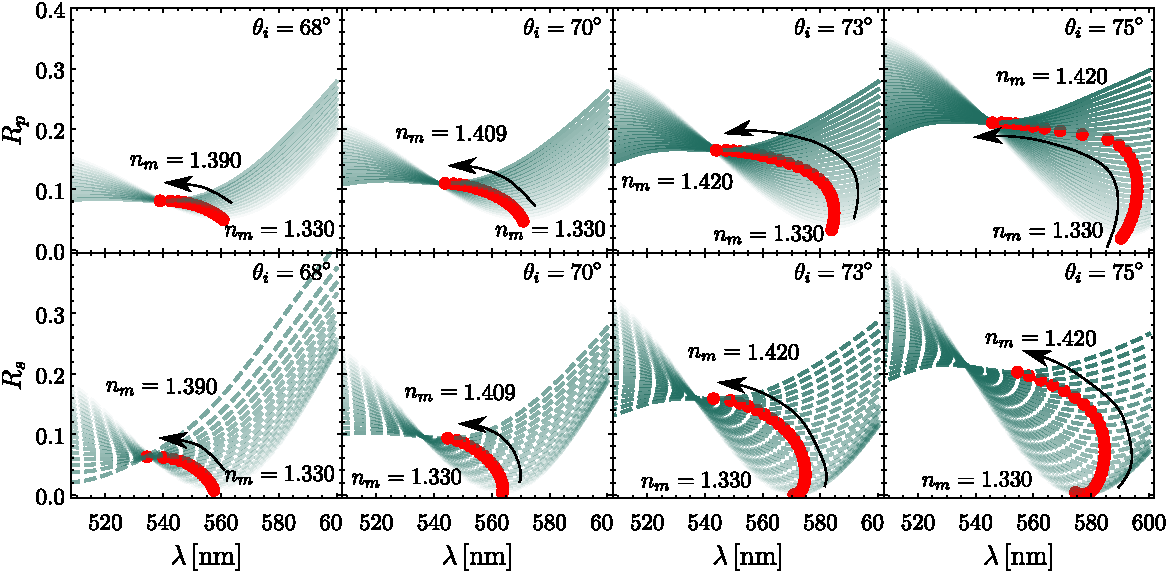
\includegraphics[width=1\linewidth]{2-Resultados/figs/11-SPPCSM/2-RpRs}\vspace*{-.7em}%
\caption{Reflectancia para polarización \emph{p}, $R_p$ (panel superior) y polarización \emph{s}, $R_s$ (panel inferior), de una monocapa desordenada de NPs de oro (radio $a=30$ nm y fracción de cubierta $\Theta=0.125$)  como función de la longitud de onda $\lambda$ para distinto valores del  índice de refracción de la matriz $n_m$. La opacidad de las gráficas es proporcional al valor de $n_m$  y los puntos rojos corresponden al mínimo de la reflectancia, es decir, al valor de $\lambda^{exc}$ considerado para los cálculos de la sensibilidad $S_B$ de la Fig. \ref{fig:SensThetai} y la tabla \ref{fig:SensRpRs}.	
	}\label{fig:SensRpRs}
	\end{figure}	

De la Fig. \ref{fig:SensRpRs} se observa que conforme el índice de refracción de la matriz aumenta, no sólo hay un corrimiento al rojo o al azul de la longitud de onda de excitación $\lambda^{exc}$  (puntos rojos en la Fig. \ref{fig:SensRpRs}) del modo colectivo,  sino también  el FWHM del supuesto modo colectivo aumenta. El supuesto modo colectivo es más sensible cuando, a un ángulo  $\theta_i$ fijo, éste se aproxima al ángulo crítico, es decir, cuando aumenta el valor de $n_m$ y se presenta un corrimiento al azul de $\lambda^{exc}$  sin embargo, es para estos casos que el FWHM aumenta, lo que puede dificultar la determinación experimental de $\lambda^{exc}$. 

Con la finalidad de determinar la calidad de un biosensor basado en el supuesto modo colectivo predicho por el CSM, se calcula la $\textit{FoM}_B$ de una moncapa desordenada de NPs esféricas de radio $a$ y fracción de cubierta $\Theta$, cuando las NPs son de oro y cuando son de plata, y se compara con la $\textit{FoM}_B$ de un sensor comercial, basado en los SPPs, para una película de oro y una de plata. En la Fig. \ref{fig:SPPCSM} se muestran los cálculos de la reflectancia en configuración ATR para una película de oro y una de plata ---donde se observa el SPP resaltado por la línea discontinua blanca---, ambas de grosor $d=50$ nm, y para una monocapa de NPs esféricas de oro (con $a=30$ nm y $\Theta=0.125$) y una de NPs de plata (con $a=40$ nm y $\Theta=0.1$) ---resaltando al supuesto modo colectivo con los puntos amarillos---; se consideró para todos los cálculo un sustrato con índice de refracción $n_s=1.5$ y una matriz de agua ($n_m=1.33$).




\begin{figure}[h!]\centering
\begin{tikzpicture}[scale=1]
\node[inner sep=0pt] (graf) at (.05,0){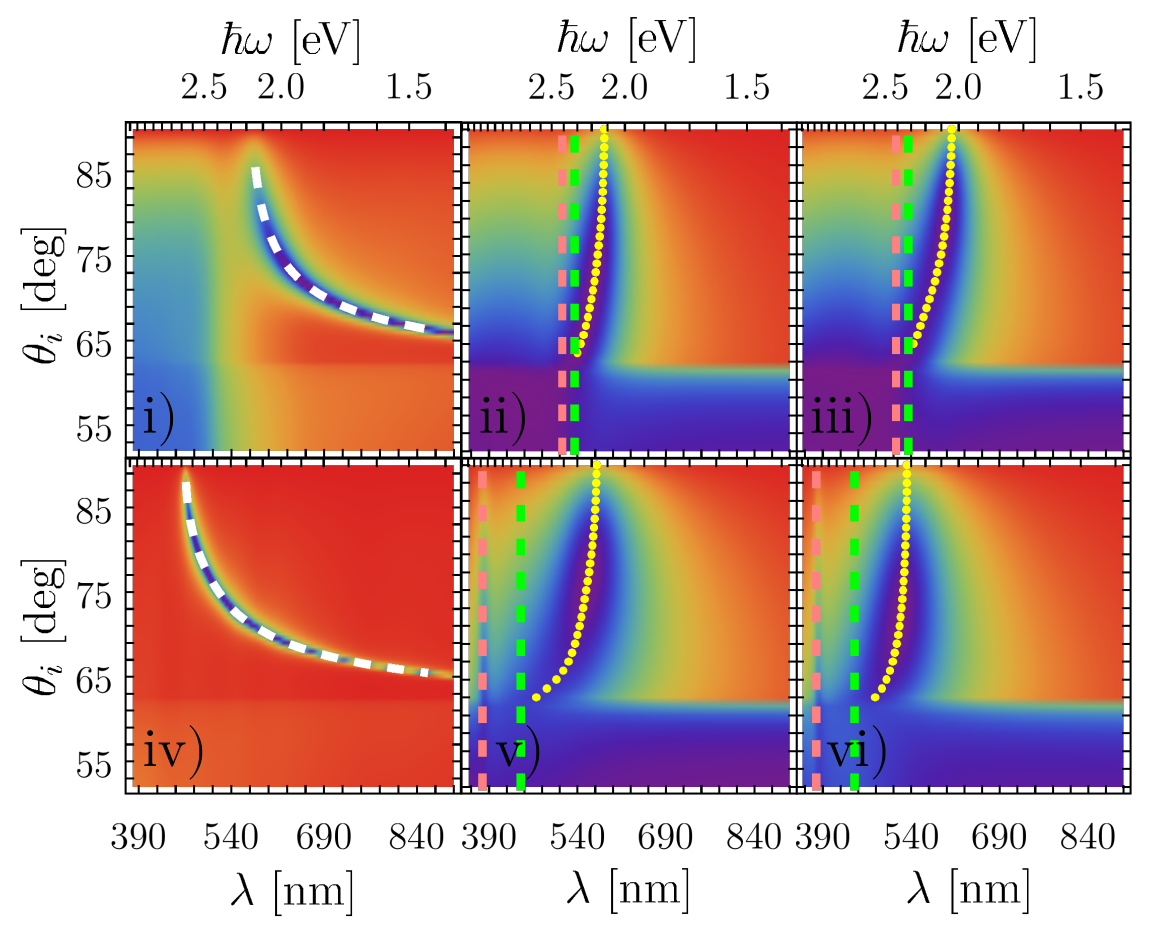
\includegraphics[scale=1]{2-Resultados/figs/11-SPPCSM/3-2D_Grid.png}};
\node[right, inner sep=0pt] (legend) at (4.4,.15) {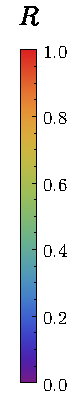
\includegraphics[scale=1, trim={00 -15 00 00}, clip]{2-Resultados/figs/0-RBar_v}};

\def\x{8}
	\node at(\x,3){\small i) SPP: Au, $d=50$ nm};
	\node at(\x,2.5){\small ii) CSM \emph{p}-Pol.:};
	\node at(\x,2.){\small \;\;\; NPs Au, $a=30$ nm, $\Theta=0.125$};	
	\node at(\x,1.5){\small iii) CSM \emph{s}-Pol.:};	
	\node at(\x,1.){\small \;\;\; NPs Au, $a=30$ nm, $\Theta=0.125$};	
			

	\node at(\x,-1){\small iv) SPP: Ag, $d=50$ nm};
	\node at(\x,-1.5){\small v) CSM \emph{p}-Pol.:};
	\node at(\x,-2){\small \;\;\;	 NPs Ag, $a=40$ nm, $\Theta=0.1$};	
	\node at(\x,-2.5){\small vi) CSM \emph{s}-Pol.:};
	\node at(\x,-3){\small \;\;\; NPs Ag, $a=40$ nm, $\Theta=0.1$};			

\def\xR{4.2}
\def\yR{2.5}	
	\node at(\xR,\yR){$R_s $};
	\node at(\xR,\yR-2.8){$R_s $};
	
	\node at(\xR-2.8,\yR){$R_p$};
	\node at(\xR-2.8,\yR-2.8){$R_p$};
	
	\node at(\xR-2*2.8,\yR){$R_p$};
	\node at(\xR-2*2.8,\yR-2.8){$R_p$};			
\end{tikzpicture}\vspace*{-.7em}
\caption{Gráficas de reflectancia $R$ en configuración ATR, considerando un sustrato con $n_m=1.5$ y una matriz acuosa $n=1.33$, como función del ángulo de incidencia $\theta_i$ y de la longitud de onda $\lambda$ (escala inferior) así como de la energía en unidades de $\hbar\omega$ (escala superior), para una película delgada de $45$ nm de grosor (columna izquierda), y una monocapa de NPs esféricas iluminada por una onda plana en polarización \emph{p} (columna central) y en polarización \emph{s} (columna derecha); los paneles superiores corresponden a una película y NPs de oro con $a=30$ nm y $\Theta=0.125$, mientras que para los inferiores corresponden a una película y NPs de plata de con $a=40$ nm y $\Theta=0.1$.  Las líneas punteadas blancas (columna izquierda) corresponde a los mínimos en la reflectancia debido a la excitación del SPP y lo puntos amarillos (columna central y columna derecha) corresponden a los mínimos en $R$ causados por el modo colectivo predicho por el CSM. Las líneas verticales punteadas verdes corresponden a la SP-SPRs dipolar ($531$ nm y $444$ nm para las NPs empleadas de oro y plata, respectivamente), y las rosas a la SP-SPR cuadrupolar ($514$ nm y $383$ nm para las NPs de oro y de plata, respectivamente).}
\label{fig:SPPCSM}
\end{figure}

En la Fig. \ref{fig:SPPCSM} se comparan las propiedades del SPP, para una película delgada de oro y una de plata, con las del supuesto modo colectivo, para una monocapa de NPs de oro y una de plata, cuando el índice de la matriz es $n_m=1.33$. El SPP, para los dos materiales considerados, no puede ser excitado dentro del espectro visible para ángulos de incidencia cercanos al crítico $\theta_c\approx 62.5^\circ$, mientras que el supuesto modo colectivo se excita para todos los ángulos de incidencia tanto para la moncapa de NPs de oro como para la de NPs de plata. Asimismo, el supuesto modo colectivo puede sintonizarse  cambiando los parámetros $\Theta$ y $a$ mas el SPP está limitado por el grosor $d$ de la película: si éste es mayor que lo longitud de penetración el SPP no puede ser excitado. Otra diferencia es el FWHM del SPP, que es menor a la del supuesto modo colectivo, para los dos materiales considerados. Al comparar el supuesto modo colectivo considerando polarización\emph{p} y \emph{s},  se observa  que el FWHM es menor para \emph{s} que para \emph{p}, tanto en las monocapas de NPs de oro como de plata; al comparar la FWHM para una polarización fija, éste es menor para las NPs de oro que para las de plata, debido al tamaño de las NPs escogida para cada monocapa.

Se grafica en la Fig. \ref{fig:FoMSPPCSM} el corrimiento al rojo de la longitud de onda de excitación $\delta\lambda^{exc}$ como función del índice de refracción $n_m$ (en un intervalo entre $1.33$ RIU y $1.332$ RIU)  del SPP [Fig. \ref{sfig:FoMSPP}], y del supuesto modo colectivo en polarización \emph{p} [Fig. \ref{sfig:FoMCSMp}] y \emph{s} [Fig. \ref{sfig:FoMCSMs}]. Se consideraron los ángulos de incidencia $\theta_i=65^\circ,\, 70^\circ,\, 75^\circ$ y $80^\circ$. Las líneas continuas corresponden a la película y la monocapa de NPs de oro, mientras que las líneas discontinuas a la película y monocapa de NPs de plata. 

La sensibilidad del SPP [Fig. \ref{sfig:FoMSPP}] sólo se reporta para $\theta_i=70^\circ,\, 75^\circ$ y $80^\circ$ dado que para $65^\circ$ el SPP no se excita en el espectro visible. Sin embargo, la sensibilidad del SPP, tanto para oro como para plata, es mayor al considerar ángulos de incidencia  menores, como se observa al comparar el corrimiento al rojo para $\theta_i=70^\circ$ (líneas amarillas) y  para $\theta_i=80^\circ$ (líneas turquesas).  Considerando un ángulo de incidencia de $70^\circ$ la sensibilidad del SPP para ambos materiales es comparable mas para $\theta_i=75^\circ$ y $80^\circ$ el SPP de la película de plata es más sensible que la del oro. El corrimiento al rojo del SPP (para oro y para plata) más amplio con los parámetros escogidos para la Fig. \ref{sfig:FoMSPP} es de $7$ nm cuando el índice de refracción de la matriz  aumenta de $1.33$ RIU a $1.332$ al considerar $\theta_i=70^\circ$.

A diferencia del SPP, el supuesto modo colectivo predicho por el CSM sí puede excitarse en el espectro visible para ángulos cercanos al ángulo crítico y, es en estos valores cuando el supuesto modo colectivo es más sensible, además de presentar un corrimiento al azul, en lugar de un corrimiento al rojo, como se observa en las Figs. \ref{sfig:FoMCSMp} y de la Fig. \ref{sfig:FoMCSMs}, para polarización \emph{p} y \emph{s}, respectivamente. El corrimiento al azul se observa para polarización \emph{p} para $\theta_i=65^\circ$ y, para este ángulo de incidencia, la monocapa de NPs de oro (línas continuas) es mayor que para la monocapa de NPs de plata (líneas discontinuas). Al considerar polarización \emph{s}, el corrimiento al azul se presenta para $\theta_i=65^\circ$ para ambos materiales sin embargo, para $\theta_i=70^\circ$ hay un corrimiento al azul para la moncapa de NPs de oro y un corrimiento al rojo para las NPs de plata. Para ambos materiales considerados y para las dos polarizaciones, cuando $\theta_i\geq 75^\circ$ el supuesto modo colectivo se corre al rojo y la sensibilidad de la monocapa de NPs de plata es mayor que para las de oro (ver líneas continuas y discontinuas del mismo color). A diferencia del SPP, la sensibilidad del supuesto modo colectivo se maximiza en dos casos: para ángulos de incidencia lo más cercanos al crítico (como también ocurre para el SPP)  y considerando ángulo de incidencia alrededor de $80^\circ$.   En las Figs. \ref{sfig:FoMCSMp} y \ref{sfig:FoMCSMs} se observa que el mayor corrimiento al rojo para el supuesto modo colectivo predicho por el CSM en polarización \emph{p} y \emph{s} es $\delta\lambda^{exc} \approx -1.5$ nm considerando $\theta_i=65^\circ$.

Con base en las Figs. \ref{fig:SPPCSM} y \ref{fig:FoMSPPCSM} se calcula la $\textit{FoM}_B$ para el SPP y el supuesto modo colectivo, presentadas en la tabla \ref{tab:FOM}. La FoM de bulto del SPP para el oro, para los ángulos de incidencia considerados, toma valores entre $48$ RIU$^{-1}$  y $70$ RIU$^{-1}$  mientras que para la plata la figura de mérito del SPP es menor, con valores entre $8$ RIU$^{-1}$ y $30$ RIU$^{-1}$. La $\textit{FoM}_B$ del supuesto modo colectivo para los cuatro ángulos de incidencia consideraros no es mayor a $5$ RIU$^{-1}$, considerando tanto el corrimiento al rojo como al azul. En la tabla \ref{tab:FOM}, se observa que a $\theta_i=65^\circ$ y a ambas polarizaciones, la $\textit{FoM}_B$ del supuesto modo colectivo presente en una monocapa de NPs de oro es menor que a $\theta_i=80^\circ$ a pesar de que la sensibilidad fue mayor para $65^\circ$ que para $80^\circ$, como se observa en las Figs. \ref{sfig:FoMCSMp} y \ref{sfig:FoMCSMs}. Esto se debe a la FWHM del supuesto modo colectivo aumenta cuando $\theta_i\approx\theta_c$, como se muestra en la Fig. \ref{fig:SensRpRs}; lo análogo sucede para la monocapa de NPs de plata. 

\begin{table}[h!]
\centering
\caption{Resultados de la figura de mérito $\textit{FoM}_B$ del SPP y del supuesto modo colectivo predicho por el CSM a ambas polarizaciones para los ángulos de incidencia $\theta_i = 65^\circ,\,70^\circ,\, 75^\circ$ y $80^\circ$. Para el SPP de consideró una película delgada de oro, y una de plata, de $50$ nm de groso y para el supuesto modo colectivo, una monocapa de NPs de oro de radio $a=30$ nm y una fracción de cubierta $\Theta=0.125$, y una monocapa de NPs de plata con $a=40$ nm y $\Theta=0.1$.}\vspace*{-.7em}
\label{tab:FOM}\small
%\resizebox{\textwidth}{!}{%
\begin{tabular}{c||c||ccc}
Au & SPP  & CSM \emph{p}-Pol. 	& CSM \emph{s}-Pol. \\ 
$\theta_i$ &  $\textit{FoM}_B$ [$\pm 0.6$ RIU$^{-1}$]	  &  $\textit{FoM}_B$ [$\pm 0.07$ RIU$^{-1}$]		&  $\textit{FoM}_B$  [$\pm 0.04$ RIU$^{-1}$]\\ \hline
$65^\circ$ & --			  &	$-2.64$ & $-0.59$\\
$70^\circ$ & $67.5$ &	$0.93$ & $1.88$\\
$75^\circ$ & $48.5$ &	$2.47$ & $3.19$\\
$80^\circ$ & $69.7$ &	$4.03$ & $4.37$\\
\hline \hline
Ag & SPP  & CSM \emph{p}-Pol. 	& CSM \emph{s}-Pol. \\ 
$\theta_i$ &  $\textit{FoM}_B$ [$\pm 0.2$ RIU$^{-1}$]	  &  $\textit{FoM}_B$ [$\pm 0.05$ RIU$^{-1}$]		&  $\textit{FoM}_B$  [$\pm 0.05$ RIU$^{-1}$]\\ \hline
$65^\circ$ & -- 			  &	$-3.66$ & $-2.08$\\
$70^\circ$ & $27.2$ &	$-0.82$ & $0.42$\\
$75^\circ$ & $12.7$ &	$1.47$  & $2.28$\\
$80^\circ$ & $8.51$ &	$3.31$  & $3.09$
\end{tabular}
\end{table}


Los resultados obtenidos para la sensibilidad y la figura de mérito de bulto del SPP son consistentes con la literatura encontrada \cite{estevez2014trends,danilov2018ultra,svedendahl2009refractometric}. Asimimso, se estima que la figura de mérito de biosensores basados en LSPRs por ejemplo para la NDs-LSPR, es del orden de la unidad \cite{svedendahl2009refractometric}, al igual que la figura de mérito de bulto calculada para el supuesto modo colectivo. A partir de estos resultados se estima que los sensores basados en SPP sean una mejor opción para el biosensado en comparación con sensores nanoestructurados. Sin embargo, se enla actualidad, la aplicación de sensores basados en NPs  se ha enfocado en el bioreconocimiento en tiempo real \cite{estevez2014trends,svedendahl2009refractometric}, es decir, en la detección de pocas partículas al rededor de la nanoestructura empleada que cambien el índice de refracción de la matriz de localmente alrededor de las NPs y no el índice de refacción de toda la matriz. 

Para caracterizar cambios locales del índice de refracción de la matriz, se emplea la sensibilidad de superfice $S_s$ dada por \cite{estevez2014trends}
%
\begin{equation}
S_s=  \frac{\delta \lambda^{exc}}{\delta d},
\end{equation}
%
en donde $\delta \lambda^{exc}$ es el corrimeinto al rojo de la longitud de onda que excita al modo empleado para el sensado y $\delta d$ el grosor de una capa  adsorbida uniformemente alrededor de la nanoestructura considerando el índice de refracción de la capa igual a la del material biológico que se desee identificar  \cite{estevez2014trends}. A partir de la $S_s$ se puede construir una FoM de superficie, la cual considera la calidad del sensado a partir de la distribución de campo cercano \cite{estevez2014trends,svedendahl2009refractometric}. Para determinar completamente si el supuesto modo colectivo, presente en una monocapa desordenada de NPs esféricas, es apto para el biosensado, se propone realizar un análisis de la  sensibilidad de superficie.


